\documentclass[journal,12pt,onecolumn]{IEEEtran}
\usepackage{cite}
 \usepackage{caption}
% \usepackage{graphicx}
\usepackage{amsmath,amssymb,amsfonts,amsthm}
\usepackage{algorithmic}
\usepackage{graphicx}
\usepackage{textcomp}
\usepackage{xcolor}
\usepackage{t
\usepackage{listings}
\usepackage{enumitem}
\usepackage{mathtools}xfonts}
\usepackage{gensymb}
\usepackage{comment}
\usepackage[breaklinks=true]{hyperref}
\usepackage{tkz-euclide} 
\usepackage{listings}
\usepackage{gvv}
%\def\inputGnumericTable{}                                 
\usepackage[latin1]{inputenc} 
\usetikzlibrary{arrows.meta, positioning}
\usepackage{xparse}
\usepackage{color}                                            
\usepackage{array}                                            
\usepackage{longtable}                                       
\usepackage{calc}                                             
\usepackage{multirow}
\usepackage{multicol}
\usepackage{hhline}                                           
\usepackage{ifthen}                                           
\usepackage{lscape}
\usepackage{tabularx}
\usepackage{array}
\usepackage{float}

\usepackage{float}
%\newcommand{\define}{\stackrel{\triangle}{=}}
\theoremstyle{remark}
\usepackage{circuitikz}
\captionsetup{justification=centering}
\usepackage{tikz}

\title{Matrices in Geometry 1.9.27}
\author{EE25BTECH11038 - GNANTHIK LUCKY}
\begin{document}
\vspace{3cm}
\maketitle
{\let\newpage\relax\maketitle}
\textbf{Question: }
Find the value of P, if the point $\vec{A}\brak{0,2}$ is equidistant from point $\vec{B}\brak{3,P}$ and $\vec{c}\brak{p,5}$

\textbf{Given: } 
$\vec{A}\myvec{0\\2}$, $\vec{B}\myvec{3\\P}$ and a point $\vec{C} \myvec{P\\ 5}$ such that $\vec{P}$ is equidistant from $\vec{A}$ and $\vec{B}$. 

\begin{align}
    \therefore \norm{\vec{A}-\vec{B}}=\norm{\vec{A}-\vec{C}}\\
    \text{On squaring both the sides, we get }\\
    \norm{\vec{A}-\vec{B}}^2=\norm{\vec{A}-\vec{C}}^2\\
    \myvec{\vec{A}-\vec{B}}^{\top}\myvec{\vec{A}-\vec{B}}=\myvec{\vec{A}-\vec{C}}^{\top}\myvec{\vec{A}-\vec{C}}\\
    \vec{A}^{\top}\vec{A} - 2\vec{A}^{\top}\vec{B} + \vec{B}^{\top}\vec{B} =\vec{A}^{\top}\vec{A} - 2\vec{A}^{\top}\vec{C} + \vec{C}^{\top}\vec{C}\\
    \norm{\vec{B}}^2 - \norm{\vec{C}}^2=2\vec{A}^{\top}\myvec{\vec{B}-\vec{C}}\\
    \norm{\myvec{3\\P}} - \norm{\myvec{P\\5}}=2\myvec{0 & 2}\myvec{3-P \\ P-5}\\
    9 + p^2 - p^2 -25 = 2\brak{0+2p-10}\\
    -16=4p - 20 \implies 4p =4 \implies p=1
\end{align}


\begin{align}
 \text{Hence, the final answer is }\fbox{p = 1}   
\end{align}
\begin{figure}[H]
    \centering
    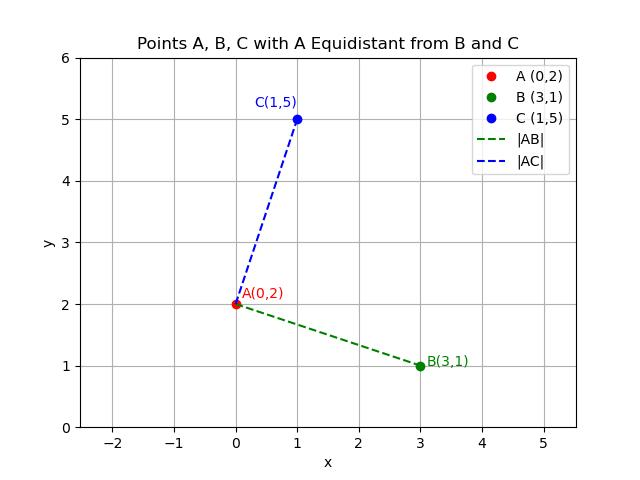
\includegraphics[width=1\columnwidth]{Figs/1.jpg}
    \caption{Plot for 1.9.27}
    \label{fig:placeholder}
\end{figure}
\end{document}